\section{Experiments}
\label{sec:exps}
We performed an extensive set of experiments to assess the effectiveness of our
model using several metrics, data sources, and model architectures, in order
to compare to prior art.

\subsection{Evaluation Metrics}
Although it is sometimes not clear whether a description should be deemed
successful or not given an image,
prior art has proposed several evaluation metrics. The most
reliable (but time consuming) is to ask for raters to give a subjective score
on the usefulness of each description given the image. In this paper, we used
this to reinforce that some of the automatic metrics indeed correlate with this
subjective score, following the guidelines proposed
in~\cite{hodosh2013framing}, which asks the
graders to evaluate each generated sentence with a scale from 1 to 4\footnote{
The raters are asked whether the image is
described without any errors, described with minor errors, with a somewhat
related description, or with an unrelated description, with a score of 4 being
the best and 1 being the worst.}.

For this metric, we set up an Amazon Mechanical Turk experiment. Each image was
rated by 2 workers. The typical level of agreement between workers
is $65\%$. In case of disagreement we simply average the scores and record the
average as the score. For variance analysis, we perform bootstrapping
(re-sampling the results with replacement and computing means/standard
deviation over the resampled results). Like~\cite{hodosh2013framing} we
report the fraction
of scores which are larger or equal than a set of predefined thresholds.

The rest of the metrics can be computed automatically assuming one has access to
groundtruth, i.e.~human generated descriptions. The most commonly used metric
so far in the image description literature has been the
BLEU score~\cite{papineni2002},
which is a form of precision of word n-grams between generated and reference
sentences~\footnote{In this literature, most previous work report BLEU-1, i.e., they only compute precision at the unigram level, whereas BLEU-n is a geometric average of precision over 1- to n-grams.}.
Even though this metric has some obvious drawbacks, it has been shown to correlate
well with human evaluations. In this work, we corroborate this as well, as
we show in Section~\ref{sec:results}. An extensive evaluation protocol, as well
as the generated outputs of our system, can be found at \url{http://nic.droppages.com/}.

Besides BLEU, one can use the perplexity of the model for a given transcription
(which is closely related to our objective function in (\ref{eqn:obj})). The perplexity
is the geometric mean of the inverse probability for each predicted word. We
used this metric to perform choices regarding model selection and hyperparameter
tuning in our held-out set, but we do not report it since BLEU is always preferred
\footnote{Even though it would be more desirable, optimizing for BLEU score yields
a discrete optimization problem. In general, perplexity and BLEU scores are fairly
correlated.}. A much more detailed discussion regarding metrics can be found in
\cite{cider}, and research groups working on this topic have been reporting
other metrics which are deemed more appropriate for evaluating caption. We report
two such metrics - METEOR and Cider - hoping for much more discussion and research
to arise regarding the choice of metric.

Lastly, the current literature on image description
has also been using the proxy task of ranking a set of available
descriptions with respect to a given image (see for instance~\cite{kiros2014}).
Doing so has the advantage that one can use known ranking metrics like recall@k.
On the other hand, transforming the description generation task into a ranking
task is unsatisfactory: as the complexity of images to describe grows, together
with its dictionary, the number of possible sentences grows exponentially with
the size of the dictionary, and
the likelihood that a predefined sentence will fit a new image will go down
unless the number of such sentences also grows exponentially, which is not
realistic; not to mention the underlying computational complexity of evaluating
efficiently such a large corpus of stored sentences for each image.
The same argument has been used in speech recognition, where one has to
produce the sentence corresponding to a given acoustic sequence; while early
attempts concentrated on classification of isolated phonemes or words,
state-of-the-art approaches for this task are now generative and can produce
sentences from a large dictionary.

Now that our models can generate descriptions of reasonable quality,
and despite the ambiguities of evaluating an image description (where there
could be multiple valid descriptions not in the groundtruth)
we believe we should concentrate on evaluation metrics for the generation task
rather than for ranking.

\subsection{Datasets}
\label{sec:data}
For evaluation we use a number of datasets which consist of images and sentences in English describing these
images. The statistics of the datasets are as follows:
\begin{center}
\begin{tabular}{|l|c|c|c|}
\hline
\multirow{2}{*}{Dataset name} & \multicolumn{3}{|c|}{size} \\
\cline{2-4}
 & train & valid. & test \\
\hline
\hline
Pascal VOC 2008 \cite{farhadi2010every} & - & - & 1000 \\
\hline
Flickr8k \cite{rashtchian2010collecting} & 6000 & 1000 & 1000 \\
\hline
Flickr30k \cite{hodoshimage} & 28000 & 1000 & 1000 \\
\hline
MSCOCO \cite{lin2014microsoft} & 82783 & 40504 & 40775 \\
\hline
SBU \cite{ordonez2011im2text} & 1M & - & - \\
\hline
\end{tabular}
\end{center}
With the exception of SBU, each image has been annotated by labelers
with 5 sentences that are
relatively visual and unbiased. SBU consists of
descriptions given by image owners when they uploaded them to Flickr. As 
such they are not guaranteed to be visual or unbiased and thus this dataset has more noise.

The Pascal dataset is customary used for testing only after a system has been trained on 
different data such as any of the other four dataset. In the case of SBU, we hold
out 1000 images for testing and train on the rest as 
used by \cite{kuznetsova2014treetalk}. Similarly, we reserve 4K random images from the
MSCOCO validation set as test, called COCO-4k, and use it to report results in the following section.


\subsection{Results}
\label{sec:results}

Since our model is data driven and trained end-to-end, and given the abundance of
datasets, we wanted to answer
questions such as ``how dataset size affects generalization'',
``what kinds of transfer learning it would be able to achieve'',
and ``how it would deal with weakly labeled examples''.
As a result, we performed experiments on five different datasets,
explained in Section~\ref{sec:data}, which enabled us to understand
our model in depth.

\subsubsection{Training Details}

Many of the challenges that we faced when training our models had to do with overfitting.
Indeed, purely supervised approaches require large amounts of data, but the datasets
that are of high quality have less than 100000 images. The task
of assigning a description is strictly harder than object classification and
data driven approaches have only recently become dominant thanks to datasets as large as ImageNet
(with ten times more data than the datasets we described in this paper, with the exception of SBU).
As a result, we believe that, even with the results we obtained which are quite good, the advantage
of our method versus most current human-engineered approaches will only increase in the next few years as training set sizes will grow.

Nonetheless, we explored several techniques to deal with overfitting. The most obvious
way to not overfit is to initialize the weights of the CNN component of our system to
a pretrained model (e.g., on ImageNet). We did this in all the experiments (similar to~\cite{gong2014improving}),
and it did help quite a lot in terms of generalization. Another set of weights that could
be sensibly initialized are $W_e$, the word embeddings. We tried initializing them
from a large news corpus~\cite{mikolov2013}, but no significant gains were observed, and we decided
to just leave them uninitialized for simplicity. Lastly, we did some model level overfitting-avoiding
techniques. We tried dropout~\cite{zaremba2014} and ensembling models, as well as exploring the size
(i.e., capacity) of the model by trading off number of hidden units versus depth. Dropout and ensembling
gave a few BLEU points improvement, and that is what we report throughout the paper.

We trained all sets of weights using stochastic gradient descent
with fixed learning rate and no momentum.
All weights were randomly initialized except for the CNN weights,
which we left unchanged because changing them had a negative impact.
We used 512 dimensions for the embeddings and the size of the LSTM memory.

Descriptions were preprocessed with basic tokenization, keeping all words
that appeared at least 5 times in the training set.

\subsubsection{Generation Results}

We report our main results on all the relevant datasets in Tables~\ref{tab:coco} and \ref{tab:bleu}.
Since PASCAL does not have a training set, we used the system trained using MSCOCO (arguably
the largest and highest quality dataset for this task). The state-of-the-art results for PASCAL
and SBU did not use image features based on deep learning, so arguably a big improvement
on those scores comes from that change alone. The Flickr datasets have been used
recently~\cite{hodosh2013framing,baidu2014,kiros2014}, but mostly evaluated in a retrieval framework. A
notable exception is~\cite{baidu2014}, where they did both retrieval and generation, and which
yields the best performance on the Flickr datasets up to now.

Human scores in Table~\ref{tab:bleu} were computed by comparing one of the human captions against the other four.
We do this for each of the five raters, and average their BLEU scores. Since this gives a slight
advantage to our system, given the BLEU score is computed against five reference sentences
and not four, we add back to the human scores the average difference of having five references instead of four.

Given that the field has seen significant advances in the last years, we do think
it is more meaningful to report BLEU-4, which is the standard in machine translation moving forward. Additionally,
we report metrics shown to correlate better with human evaluations in Table~\ref{tab:coco}\footnote{We
used the implementation of these metrics kindly provided in \url{http://www.mscoco.org}.}.
Despite recent efforts on better evaluation metrics \cite{cider}, our model fares strongly versus
human raters. However, when evaluating our captions using human raters (see Section~\ref{sec:human}),
our model fares much more poorly, suggesting more work is needed towards better metrics.
On the official test set for which labels are only available through the official website, our model had a 27.2 BLEU-4.

\begin{table}
\centering
\begin{small}
\begin{tabular}{|c|c|c|c|}
 \hline
Metric & BLEU-4 & METEOR & CIDER \\
\hline
\hline
NIC   & \bf{27.7}  & \bf{23.7} & \bf{85.5}     \\
\hline
Random  &   4.6    &  9.0    &  5.1    \\
Nearest Neighbor & 9.9  & 15.7  & 36.5   \\
Human   & 21.7  & 25.2 & 85.4 \\
\hline
\end{tabular}
\end{small}
\caption{Scores on the MSCOCO development set.}\label{tab:coco}
\end{table}

\begin{table}
\centering
\begin{small}
\begin{tabular}{|c|c|c|c|c|}
 \hline
Approach & PASCAL & Flickr& Flickr& SBU  \\
         & (xfer) & 30k   & 8k    &      \\
\hline
\hline
Im2Text~\cite{ordonez2011im2text} &     &     &     & 11     \\
TreeTalk~\cite{kuznetsova2014treetalk} &     &     &     & 19     \\
BabyTalk~\cite{kulkarni2011baby} & 25  &     &     &        \\
Tri5Sem~\cite{hodosh2013framing} &     &     & 48  &        \\
m-RNN~\cite{baidu2014} &     & 55  & 58  &        \\
MNLM~\cite{kiros2014}\footnotemark &     & 56  & 51  &        \\
\hline
SOTA      & 25  & 56  & 58  & 19     \\
\hline
NIC   & \bf{59}  & \bf{66} & \bf{63}  & \bf{28}     \\
\hline
Human   & 69  & 68 & 70  &        \\
\hline
\end{tabular}
\end{small}
\caption{BLEU-1 scores. We only report previous work
results when available. SOTA stands for the current
state-of-the-art.}\label{tab:bleu}
\end{table}

\footnotetext{We computed these BLEU scores with the outputs that the authors of \cite{kiros2014} kindly provided for their OxfordNet system.}

\subsubsection{Transfer Learning, Data Size and Label Quality}

Since we have trained many models and we have several testing sets, we wanted to
study whether we could transfer a model to a different dataset, and how much the
mismatch in domain would be compensated with e.g. higher quality labels or more training
data.

The most obvious case for transfer learning and data size is between Flickr30k and Flickr8k. The two
datasets are similarly labeled as they were created by the same group.
Indeed, when training on Flickr30k (with about 4 times more training data),
the results obtained are 4 BLEU points better.
It is clear that in this case, we see gains by adding more training data
since the whole process is data-driven and overfitting prone.
MSCOCO is even bigger (5 times more
training data than Flickr30k), but since the collection process was done differently, there are likely
more differences in vocabulary and a larger mismatch. Indeed, all the BLEU scores degrade by 10 points.
Nonetheless, the descriptions are still reasonable.

Since PASCAL has no official training set and was collected independently of Flickr and MSCOCO, we
report transfer learning from MSCOCO (in Table~\ref{tab:bleu}). Doing transfer learning from
Flickr30k yielded worse results with BLEU-1 at 53 (cf. 59).

Lastly, even though SBU has weak labeling (i.e., the labels were captions and not
human generated descriptions), the task is much harder with a much larger and noisier
vocabulary. However, much more data is available for training. When running the MSCOCO
model on SBU, our performance degrades from 28 down to 16.

\subsubsection{Generation Diversity Discussion}

Having trained a generative model that gives $p(S|I)$, an obvious question is
whether the model generates novel captions, and whether the generated captions
are both diverse and high quality.
Table~\ref{tab:diversity} shows some samples when returning the N-best list from our
beam search decoder instead of the best hypothesis. Notice how the samples are
diverse and may show different aspects from the same image.
The agreement in BLEU score between the top 15 generated sentences is 58, which is similar to that of humans among them. This indicates the amount of diversity
our model generates.
In bold are the sentences that
are not present in the training set. If we take the best candidate, the
sentence is present in the training set 80\% of the times.
This is not too surprising given that the amount
of training data is quite small, so it is relatively easy for the model to pick ``exemplar''
sentences and use them to generate descriptions.
If we instead analyze the top 15 generated sentences, about half of the times we
see a completely novel description, but still with a similar BLEU score,
indicating that they are of enough quality, yet they
provide a healthy diversity.

\begin{table}[htb]
\begin{center}
\begin{tabular}{|l|}\hline
A man throwing a frisbee in a park. \\
{\bf A man holding a frisbee in his hand.} \\
{\bf A man standing in the grass with a frisbee.} \\
\hline
A close up of a sandwich on a plate. \\
A close up of a plate of food with french fries. \\
A white plate topped with a cut in half sandwich. \\
\hline
A display case filled with lots of donuts. \\
{\bf A display case filled with lots of cakes.} \\
{\bf A bakery display case filled with lots of donuts.} \\
\hline
\end{tabular}
\end{center}
\caption{{N-best examples from the MSCOCO test set. Bold lines indicate a novel sentence not present in the training set.}}
\label{tab:diversity}
\end{table}

\subsubsection{Ranking Results}

While we think ranking is an unsatisfactory way to evaluate description
generation from images, many papers report ranking scores,
using the set of testing captions as candidates to rank given a test image.
The approach that works best on these metrics (MNLM),
specifically implemented a ranking-aware loss. Nevertheless,
NIC is doing surprisingly well on both ranking tasks (ranking descriptions
given images, and ranking images given descriptions),
as can be seen in
Tables~\ref{tab:recall@10} and~\ref{tab:recall@1030k}. Note that for the Image Annotation task, we normalized our scores similar to what~\cite{baidu2014} used.

\begin{table}
\centering
\begin{small}
\setlength{\tabcolsep}{3pt}
\begin{tabular}{|c|ccc|ccc|}
 \hline
\multirow{2}{*}{Approach} & \multicolumn{3}{c|}{Image Annotation} & \multicolumn{3}{c|}{Image Search} \\
 & R@1 & R@10 & Med $r$ &  R@1 & R@10 & Med $r$ \\
\hline
\hline
DeFrag~\cite{karpathy2014deep} & 13 & 44 & 14             &    10 & 43 & 15  \\
m-RNN~\cite{baidu2014}         &  15 & 49 & 11               &  12 & 42 & 15\\
MNLM~\cite{kiros2014}        &  18   & 55 & 8        &  13 & 52 & 10   \\
\hline
NIC                            &  \bf{20} & \bf{61} & \bf{6}              &    \bf{19} & \bf{64} & \bf{5} \\
\hline
\end{tabular}
\end{small}
\caption{Recall@k and median rank on Flickr8k.\label{tab:recall@10}}
\end{table}

\begin{table}
\centering
\begin{small}
\setlength{\tabcolsep}{3pt}
\begin{tabular}{|c|ccc|ccc|}
\hline
\multirow{2}{*}{Approach} & \multicolumn{3}{c|}{Image Annotation} & \multicolumn{3}{c|}{Image Search} \\
 & R@1 & R@10 & Med $r$ &  R@1 & R@10 & Med $r$ \\
\hline
\hline
DeFrag~\cite{karpathy2014deep} & 16 & 55 & 8             &    10 & 45 & 13  \\
m-RNN~\cite{baidu2014}         &  18 & 51 & 10               &  13 & 42 & 16\\
MNLM~\cite{kiros2014}        &  \bf{23}   & \bf{63} & \bf{5}        &  \bf{17} & \bf{57} & \bf{8}   \\
\hline
NIC                            &  17 & 56  & 7               &    \bf{17} & \bf{57} & \bf{7} \\
\hline
\end{tabular}
\end{small}
\caption{Recall@k and median rank on Flickr30k.\label{tab:recall@1030k}}
\end{table}


\subsubsection{Human Evaluation}
\label{sec:human}

Figure~\ref{fig:turk_eval_numeric} shows the result of the human evaluations
of the descriptions provided by NIC, as well as a reference system and
groundtruth on various datasets. We can see that NIC is better than the reference
system, but clearly worse than the groundtruth, as expected.
This shows that BLEU is not a perfect metric, as it does not capture well
the difference between NIC and human descriptions assessed by raters.
Examples of rated images can be seen in Figure~\ref{fig:turk_eval_examples}.
It is interesting to see, for instance in the second image of the first
column, how the model was able to notice the frisbee given its size.

\begin{figure}
\begin{center}
  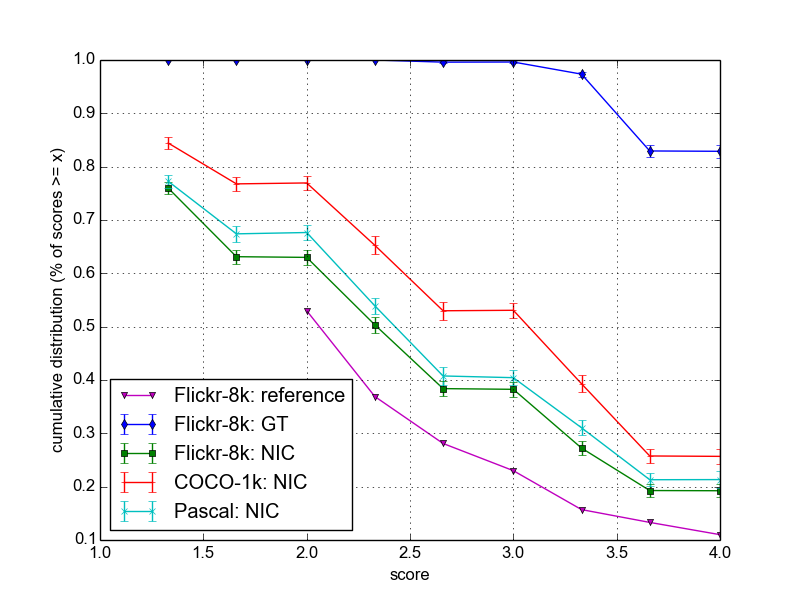
\includegraphics[width=1.0\columnwidth]{turk_eval}
\end{center}
\vspace{-0.5cm}
\caption{\label{fig:turk_eval_numeric} {\em Flickr-8k: NIC}: predictions produced by NIC on the Flickr8k test set (average score: 2.37); {\em Pascal: NIC}: (average score: 2.45); {\em COCO-1k: NIC}: A subset of 1000 images from the MSCOCO test set with descriptions produced by NIC (average score: 2.72); {\em Flickr-8k: ref}: these are results from~\cite{hodosh2013framing} on Flickr8k rated using the same protocol, as a baseline (average score: 2.08); {\em Flickr-8k: GT}: we rated the groundtruth labels from Flickr8k using the same protocol. This provides us with a ``calibration'' of the scores (average score: 3.89)}
\end{figure}

\begin{figure*}
\begin{center}
  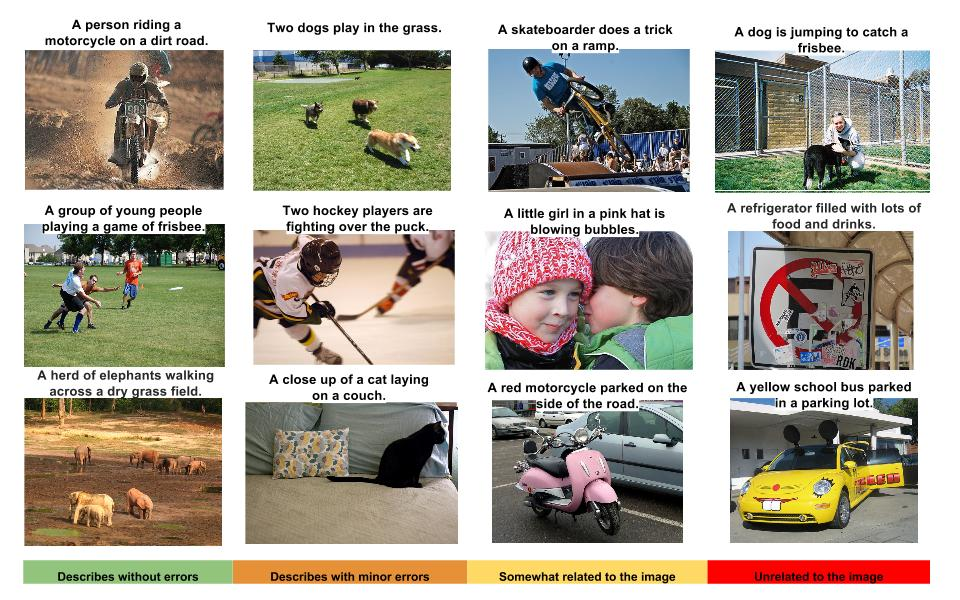
\includegraphics[width=\textwidth]{nic_rated.jpg}
\vspace{-1cm}
\end{center}
\caption{\label{fig:turk_eval_examples} A selection of evaluation results, grouped by human rating.}
\end{figure*}


\subsubsection{Analysis of Embeddings}

In order to represent the previous word $S_{t-1}$ as input to the decoding LSTM
producing $S_t$, we use word embedding vectors~\cite{mikolov2013},
which have the advantage of
being independent of the size of the dictionary (contrary to a simpler
one-hot-encoding approach).
Furthermore, these word embeddings can be jointly trained with the rest of the
model. It is remarkable to see how the learned representations
have captured some semantic from the statistics of the language.
Table~\ref{tab:embeddings} shows, for a few example words, the nearest other
words found in the learned embedding space.

Note how some of the relationships
learned by the model will help the vision component. Indeed, having ``horse'', ``pony'',
and ``donkey'' close to each other will encourage the CNN to extract features that
are relevant to horse-looking animals.
We hypothesize that, in the extreme case where we see very few examples of a class (e.g., ``unicorn''),
its proximity to other word embeddings (e.g., ``horse'') should
provide a lot more information that would be completely lost with more
traditional bag-of-words based approaches.


\begin{table}[htb]
\label{tab:embeddings}
\begin{center}
\begin{tabular}{|l|l|}\hline
Word & Neighbors \\ \hline
car & van, cab, suv, vehicule, jeep \\
boy & toddler, gentleman, daughter, son \\
street & road, streets, highway, freeway \\
horse & pony, donkey, pig, goat, mule \\
computer & computers, pc, crt, chip, compute \\ \hline
\end{tabular}
\end{center}
\caption{{Nearest neighbors of a few example words}}
\end{table}


